\documentclass[11pt]{article}
\usepackage[a4paper,landscape,margin=0.72in]{geometry}
\usepackage[T1]{fontenc}
\usepackage{lmodern,amsmath,amssymb,graphicx,hyperref}
\title{Source-style common 2+2 norm in the actual rational-point stalk}
\author{Formal proof packet}
\date{28 October 2026}
\begin{document}
\maketitle
\noindent This packet records checked algebraic transport and a conditional local-order corollary. It contains no target result, experiment, or cost ratio. The Lean source, compiler log, editable SVG, and CSV gate table accompany this PDF.

\section*{Checked boundary}
For a rational point $y^2=f(a)$ on the actual monic quintic chart, the checked ring map sends the quintic $f(X)$ to $Y^2$ in the weighted-$\operatorname{Proj}$ point stalk. Consequently a polynomial identity $n^2-u_1u_2U=b^2f$ maps to
\[
  (n(X)-bY)(n(X)+bY)=u_1(X)u_2(X)U(X)
\]
in that actual stalk. The source-style common 2+2 theorem supplies this identity under explicit valid Mumford congruences and a nonzero interpolation determinant. This algebraic transport needs neither a DVR nor odd characteristic.

The separate checked \texttt{projective\_norm\_order} theorem uses the actual nonbranch DVR when $f$ is separable, $2y\ne0$, and $b\ne0$. If the chosen factor $n(X)-bY$ is a nonunit, the other conjugate factor is a unit, so its order is the sum of the $u_1,u_2,U$ orders. The polynomial identity and chosen-factor nonunit premise are explicit. The source-style identity and generic order theorem have not yet been combined into a single source-style order wrapper.

\section*{Exceptional boundary and verification}
In characteristic two the conjugate factors coincide, since $n-bY=n+bY$. The norm identity still transports, but this order-allocation argument does not apply even at derivative-smooth points. Branch points with $y=0$ use the separate checked branch analysis.

Direct pinned Lean 4.34.1 compilation exited zero against Mathlib revision
\par\noindent\texttt{d13f23b723b8a846827a245b89c10fc7d3f11612}.
Four printed axiom audits list only \texttt{propext}, \texttt{Classical.choice}, and \texttt{Quot.sound}; no \texttt{sorryAx}. Source SHA-256:
\par\noindent{\small\texttt{601f8714b191f015d76d477cb1eb590014097281de538abe56d693f19288d52d}}.
The local DVR criterion follows pinned Mathlib \texttt{IsDiscreteValuationRing.TFAE} and Stacks Project Tag 00PD. Global principal-divisor/$\mathrm{Pic}^0$ transport and compiled Rust semantics remain open.

\clearpage
\section*{Proof dependencies and open gates}
\begin{center}
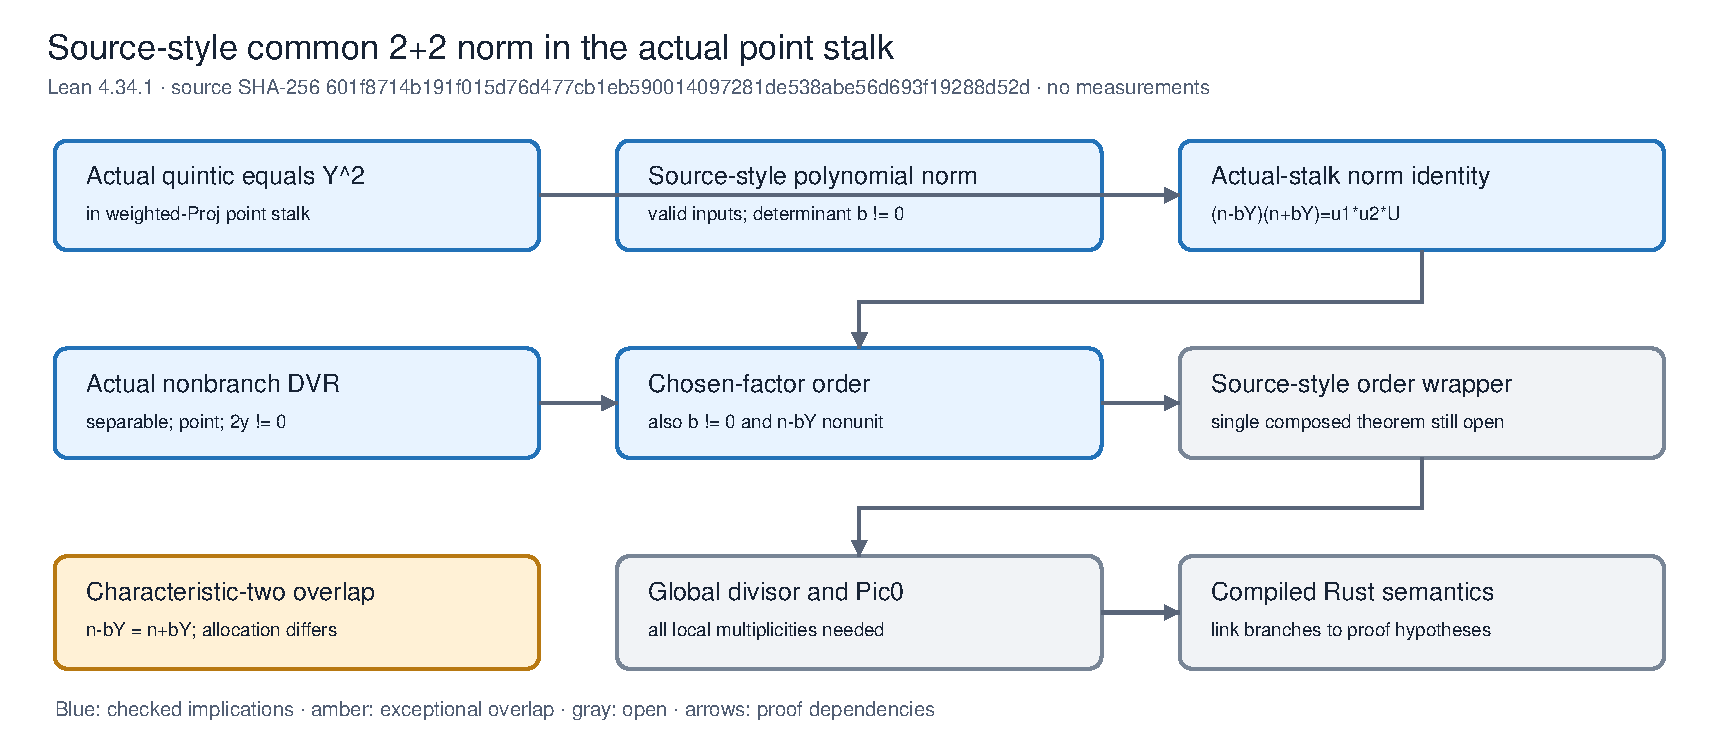
\includegraphics[width=0.96\textwidth,height=0.76\textheight,keepaspectratio]{nonbranch-norm-transport-figure.pdf}
\end{center}
\noindent Blue nodes are checked implications. Amber marks characteristic-two overlap; gray nodes remain open. Arrows show proof dependencies, not measured performance.
\end{document}
